\documentclass[a4paper]{article}

%% Language and font encodings
\usepackage[english]{babel}
\usepackage[utf8]{inputenc}
\usepackage[T1]{fontenc}

%% Sets page size and margins
\usepackage[a4paper,top=3cm,bottom=2cm,left=3cm,right=3cm,marginparwidth=1.75cm]{geometry}

%% Useful packages
\usepackage[tbtags]{amsmath}
\usepackage{mathtools}
\usepackage{graphicx}
\usepackage[colorinlistoftodos]{todonotes}
\usepackage[colorlinks=true, allcolors=blue]{hyperref}
\usepackage{color}
\usepackage{tikz}
\usepackage{titlesec}
\usepackage{caption}
\usepackage[shortlabels]{enumitem}
\usepackage{setspace}
\usepackage{authblk}
\usepackage{floatrow}

\floatstyle{plaintop}
\restylefloat{table}

\usetikzlibrary{shapes.geometric, arrows}

% package to manage citations
\usepackage[backend=bibtex,style=authoryear-comp,sorting=nyt,isbn=false,url=false, natbib=true, doi=false]{biblatex}
\addbibresource{bibliography.bib}

\tikzstyle{startstop_big} = [rectangle, rounded corners, minimum width=3cm, minimum height=1cm,text centered, draw=black,text width = 8.5cm, fill=red!30]
\tikzstyle{startstop} = [rectangle, rounded corners, minimum width=3cm, minimum height=1cm,text centered, draw=black,text width = 5cm, fill=red!30]
\tikzstyle{io} = [trapezium, trapezium left angle=70, trapezium right angle=110, minimum width=2cm, minimum height=1cm, text centered, draw=black, fill=blue!30]
\tikzstyle{process} = [rectangle, minimum width=3cm, minimum height=1cm, text centered, text width = 3cm, draw=black, fill=orange!30]
\tikzstyle{process_wide_3pt5cm} = [rectangle, minimum width=3cm, minimum height=1cm, text centered, text width = 3.5cm, draw=black, fill=orange!30]
\tikzstyle{process_wide_4cm} = [rectangle, minimum width=3cm, minimum height=1cm, text centered, text width = 4cm, draw=black, fill=orange!30]
\tikzstyle{process_wide_4pt5cm} = [rectangle, minimum width=3cm, minimum height=1cm, text width = 4.5cm, draw=black, fill=orange!30]
\tikzstyle{process_wide_5cm} = [rectangle, minimum width=3cm, minimum height=1cm, text width = 5cm, draw=black, fill=orange!30]
\tikzstyle{decision} = [diamond, minimum width=1cm, minimum height=1cm,text centered,text width = 2.25cm, draw=black, fill=green!30]
\tikzstyle{arrow} = [thick,->,>=stealth]


\definecolor{ErasmusBlue}{RGB}{12, 32, 116}

%Use 4 levels of sections using package titlesec
%\setcounter{secnumdepth}{4}
\newcommand{\subsubsubsection}[1]{\paragraph{#1}\mbox{}\\\\}
\newcommand*\diff{\mathop{}\!\mathrm{d}}
%\newcommand{\argmax}[1]{\underset{#1}{\operatorname{arg}\,\operatorname{max}}\;}
\DeclareMathOperator{\argmax}{arg\,max}
\DeclarePairedDelimiter\abs{\lvert}{\rvert}%
\DeclarePairedDelimiter\norm{\lVert}{\rVert}%

\let\bmath\boldsymbol
\let\rmn\mathrm
\newcommand{\Hline}
{
\hline
\hline
}


\begin{document}
\title{\textbf{Personalized Schedules for Surveillance of Low Risk Prostate Cancer Patients}}

\author[1,*]{Anirudh Tomer}
\author[2]{Daan Nieboer }
\author[3]{Monique J. Roobol }
\author[2,4]{Ewout W. Steyerberg }
\author[1]{Dimitris Rizopoulos}
\affil[1]{Department of Biostatistics, Erasmus University Medical Center, the Netherlands}
\affil[2]{Department of Public Health, Erasmus University Medical Center, the Netherlands}
\affil[3]{Department of Urology, Erasmus University Medical Center, the Netherlands}
\affil[4]{Department of Medical Statistics and Bioinformatics, Leiden University Medical Center, the Netherlands}
\affil[ ]{*\textit {email}: a.tomer@erasmusmc.nl}

\date{}

\maketitle

  In this paper, we explore the connection between secret key agreement and secure omniscience within the setting of the multiterminal source model with a wiretapper who has side information. While the secret key agreement problem considers the generation of a maximum-rate secret key through public discussion, the secure omniscience problem is concerned with communication protocols for omniscience that minimize the rate of information leakage to the wiretapper. The starting point of our work is a lower bound on the minimum leakage rate for omniscience, $\rl$, in terms of the wiretap secret key capacity, $\wskc$. Our interest is in identifying broad classes of sources for which this lower bound is met with equality, in which case we say that there is a duality between secure omniscience and secret key agreement. We show that this duality holds in the case of certain finite linear source (FLS) models, such as two-terminal FLS models and pairwise independent network models on trees with a linear wiretapper. Duality also holds for any FLS model in which $\wskc$ is achieved by a perfect linear secret key agreement scheme. We conjecture that the duality in fact holds unconditionally for any FLS model. On the negative side, we give an example of a (non-FLS) source model for which duality does not hold if we limit ourselves to communication-for-omniscience protocols with at most two (interactive) communications.  We also address the secure function computation problem and explore the connection between the minimum leakage rate for computing a function and the wiretap secret key capacity.
  
%   Finally, we demonstrate the usefulness of our lower bound on $\rl$ by using it to derive equivalent conditions for the positivity of $\wskc$ in the multiterminal model. This extends a recent result of Gohari, G\"{u}nl\"{u} and Kramer (2020) obtained for the two-user setting.
  
   
%   In this paper, we study the problem of secret key generation through an omniscience achieving communication that minimizes the 
%   leakage rate to a wiretapper who has side information in the setting of multiterminal source model.  We explore this problem by deriving a lower bound on the wiretap secret key capacity $\wskc$ in terms of the minimum leakage rate for omniscience, $\rl$. 
%   %The former quantity is defined to be the maximum secret key rate achievable, and the latter one is defined as the minimum possible leakage rate about the source through an omniscience scheme to a wiretapper. 
%   The main focus of our work is the characterization of the sources for which the lower bound holds with equality \textemdash it is referred to as a duality between secure omniscience and wiretap secret key agreement. For general source models, we show that duality need not hold if we limit to the communication protocols with at most two (interactive) communications. In the case when there is no restriction on the number of communications, whether the duality holds or not is still unknown. However, we resolve this question affirmatively for two-user finite linear sources (FLS) and pairwise independent networks (PIN) defined on trees, a subclass of FLS. Moreover, for these sources, we give a single-letter expression for $\wskc$. Furthermore, in the direction of proving the conjecture that duality holds for all FLS, we show that if $\wskc$ is achieved by a \emph{perfect} secret key agreement scheme for FLS then the duality must hold. All these results mount up the evidence in favor of the conjecture on FLS. Moreover, we demonstrate the usefulness of our lower bound on $\wskc$ in terms of $\rl$ by deriving some equivalent conditions on the positivity of secret key capacity for multiterminal source model. Our result indeed extends the work of Gohari, G\"{u}nl\"{u} and Kramer in two-user case.
%\doublespacing
% \leavevmode
% \\
% \\
% \\
% \\
% \\
\section{Introduction}
\label{introduction}

AutoML is the process by which machine learning models are built automatically for a new dataset. Given a dataset, AutoML systems perform a search over valid data transformations and learners, along with hyper-parameter optimization for each learner~\cite{VolcanoML}. Choosing the transformations and learners over which to search is our focus.
A significant number of systems mine from prior runs of pipelines over a set of datasets to choose transformers and learners that are effective with different types of datasets (e.g. \cite{NEURIPS2018_b59a51a3}, \cite{10.14778/3415478.3415542}, \cite{autosklearn}). Thus, they build a database by actually running different pipelines with a diverse set of datasets to estimate the accuracy of potential pipelines. Hence, they can be used to effectively reduce the search space. A new dataset, based on a set of features (meta-features) is then matched to this database to find the most plausible candidates for both learner selection and hyper-parameter tuning. This process of choosing starting points in the search space is called meta-learning for the cold start problem.  

Other meta-learning approaches include mining existing data science code and their associated datasets to learn from human expertise. The AL~\cite{al} system mined existing Kaggle notebooks using dynamic analysis, i.e., actually running the scripts, and showed that such a system has promise.  However, this meta-learning approach does not scale because it is onerous to execute a large number of pipeline scripts on datasets, preprocessing datasets is never trivial, and older scripts cease to run at all as software evolves. It is not surprising that AL therefore performed dynamic analysis on just nine datasets.

Our system, {\sysname}, provides a scalable meta-learning approach to leverage human expertise, using static analysis to mine pipelines from large repositories of scripts. Static analysis has the advantage of scaling to thousands or millions of scripts \cite{graph4code} easily, but lacks the performance data gathered by dynamic analysis. The {\sysname} meta-learning approach guides the learning process by a scalable dataset similarity search, based on dataset embeddings, to find the most similar datasets and the semantics of ML pipelines applied on them.  Many existing systems, such as Auto-Sklearn \cite{autosklearn} and AL \cite{al}, compute a set of meta-features for each dataset. We developed a deep neural network model to generate embeddings at the granularity of a dataset, e.g., a table or CSV file, to capture similarity at the level of an entire dataset rather than relying on a set of meta-features.
 
Because we use static analysis to capture the semantics of the meta-learning process, we have no mechanism to choose the \textbf{best} pipeline from many seen pipelines, unlike the dynamic execution case where one can rely on runtime to choose the best performing pipeline.  Observing that pipelines are basically workflow graphs, we use graph generator neural models to succinctly capture the statically-observed pipelines for a single dataset. In {\sysname}, we formulate learner selection as a graph generation problem to predict optimized pipelines based on pipelines seen in actual notebooks.

%. This formulation enables {\sysname} for effective pruning of the AutoML search space to predict optimized pipelines based on pipelines seen in actual notebooks.}
%We note that increasingly, state-of-the-art performance in AutoML systems is being generated by more complex pipelines such as Directed Acyclic Graphs (DAGs) \cite{piper} rather than the linear pipelines used in earlier systems.  
 
{\sysname} does learner and transformation selection, and hence is a component of an AutoML systems. To evaluate this component, we integrated it into two existing AutoML systems, FLAML \cite{flaml} and Auto-Sklearn \cite{autosklearn}.  
% We evaluate each system with and without {\sysname}.  
We chose FLAML because it does not yet have any meta-learning component for the cold start problem and instead allows user selection of learners and transformers. The authors of FLAML explicitly pointed to the fact that FLAML might benefit from a meta-learning component and pointed to it as a possibility for future work. For FLAML, if mining historical pipelines provides an advantage, we should improve its performance. We also picked Auto-Sklearn as it does have a learner selection component based on meta-features, as described earlier~\cite{autosklearn2}. For Auto-Sklearn, we should at least match performance if our static mining of pipelines can match their extensive database. For context, we also compared {\sysname} with the recent VolcanoML~\cite{VolcanoML}, which provides an efficient decomposition and execution strategy for the AutoML search space. In contrast, {\sysname} prunes the search space using our meta-learning model to perform hyperparameter optimization only for the most promising candidates. 

The contributions of this paper are the following:
\begin{itemize}
    \item Section ~\ref{sec:mining} defines a scalable meta-learning approach based on representation learning of mined ML pipeline semantics and datasets for over 100 datasets and ~11K Python scripts.  
    \newline
    \item Sections~\ref{sec:kgpipGen} formulates AutoML pipeline generation as a graph generation problem. {\sysname} predicts efficiently an optimized ML pipeline for an unseen dataset based on our meta-learning model.  To the best of our knowledge, {\sysname} is the first approach to formulate  AutoML pipeline generation in such a way.
    \newline
    \item Section~\ref{sec:eval} presents a comprehensive evaluation using a large collection of 121 datasets from major AutoML benchmarks and Kaggle. Our experimental results show that {\sysname} outperforms all existing AutoML systems and achieves state-of-the-art results on the majority of these datasets. {\sysname} significantly improves the performance of both FLAML and Auto-Sklearn in classification and regression tasks. We also outperformed AL in 75 out of 77 datasets and VolcanoML in 75  out of 121 datasets, including 44 datasets used only by VolcanoML~\cite{VolcanoML}.  On average, {\sysname} achieves scores that are statistically better than the means of all other systems. 
\end{itemize}


%This approach does not need to apply cleaning or transformation methods to handle different variances among datasets. Moreover, we do not need to deal with complex analysis, such as dynamic code analysis. Thus, our approach proved to be scalable, as discussed in Sections~\ref{sec:mining}.
% !TEX root =  ../pers_schedules.tex 
\section{Joint Model for Time to Event and Longitudinal Outcomes}
\label{sec : jm_framework}
We start with the definition of the joint modeling framework that will be used to fit a model to the available dataset, and then to plan biopsies for future patients. Let $T_i^*$ denote the true GR time for the $i$-th patient enrolled in an AS program. Let $S$ be the schedule of biopsies prescribed to this patient. The corresponding vector of time of biopsies is denoted by $T_i^S = \{T^S_{i0}, T^S_{i1}, \ldots, T^S_{i{N_i^S}}; T^S_{ij} < T^S_{ik}, \forall j<k\}$, where $N_i^S$ are the total number of biopsies conducted. Because of the periodical nature of biopsy schedules, $T_i^*$ cannot be observed directly and it is only known to fall in an interval $l_i < T_i^* \leq r_i$, where $l_i = T^S_{i{N_i^S - 1}}, r_i = T^S_{i{N_i^S}}$ if GR is observed, and $l_i = T^S_{i{N_i^S}}, r_i=\infty$ if GR is not observed yet. Further let $\bmath{y}_i$ denote the $n_i \times 1$  vector of PSA levels for the $i$-th patient. For a sample of $n$ patients the observed data is denoted by $\mathcal{D}_n = \{l_i, r_i, \bmath{y}_i; i = 1, \ldots, n\}$.

The longitudinal outcome of interest, namely PSA level, is continuous in nature and thus to model it the joint model utilizes a linear mixed effects model (LMM) of the form:
\begin{equation*}
\begin{split}
y_i(t) &= m_i(t) + \varepsilon_i(t)\\
&=\bmath{x}_i^T(t) \bmath{\beta} + \bmath{z}_i^T(t) \bmath{b}_i + \varepsilon_i(t),
\end{split}
\end{equation*}
where $\bmath{x}_i(t)$ denotes the row vector of the design matrix for fixed effects and $\bmath{z}_i(t)$ denotes the same for random effects. Correspondingly the fixed effects are denoted by $\bmath{\beta}$ and random effects by $\bmath{b}_i$. The random effects are assumed to be normally distributed with mean zero and $q \times q$ covariance matrix $\bmath{D}$. The true and unobserved PSA level at time $t$ is denoted by $m_i(t)$. Unlike $y_i(t)$, the former is not contaminated with the measurement error $\varepsilon_i(t)$. The error is assumed to be normally distributed with mean zero and variance $\sigma^2$, and is independent of the random effects $\bmath{b}_i$.

To model the effect of PSA on hazard of GR, joint models utilize a relative risk sub-model. The hazard of GR for patient $i$ at any time point $t$, denoted by $h_i(t)$, depends on a function of subject specific linear predictor $m_i(t)$ and/or the random effects:
\begin{align*}
h_i(t \mid \mathcal{M}_i(t), \bmath{w}_i) &= \lim_{\Delta t \to 0} \frac{\mbox{Pr}\big\{t \leq T^*_i < t + \Delta t \mid T^*_i \geq t, \mathcal{M}_i(t), \bmath{w}_i\big\}}{\Delta t}\\
&=h_0(t) \exp\big[\bmath{\gamma}^T\bmath{w}_i + f\{M_i(t), \bmath{b}_i, \bmath{\alpha}\}\big], \quad t>0,
\end{align*}
where $\mathcal{M}_i(t) = \{m_i(v), 0\leq v \leq t\}$ denotes the history of the underlying PSA levels up to time $t$. The vector of baseline covariates is denoted by $\bmath{w}_i$, and $\bmath{\gamma}$ are the corresponding parameters. The function $f(\cdot)$ parametrized by vector $\bmath{\alpha}$ specifies the functional form of PSA levels \citep{brown2009assessing,rizopoulos2012joint,taylor2013real,rizopoulos2014bma} that is used in the linear predictor of the relative risk model. Some functional forms relevant to the problem at hand are the following: 
\begin{eqnarray*}
\left \{
\begin{array}{l}
f\{M_i(t), \bmath{b}_i, \bmath{\alpha}\} = \alpha m_i(t),\\
f\{M_i(t), \bmath{b}_i, \bmath{\alpha}\} = \alpha_1 m_i(t) + \alpha_2 m'_i(t),\quad \text{with}\  m'_i(t) = \frac{\rmn{d}{m_i(t)}}{\rmn{d}{t}}.\\
\end{array}
\right.
\end{eqnarray*}
These formulations of $f(\cdot)$ postulate that the hazard of GR at time $t$ may be associated with the underlying level $m_i(t)$ of the PSA at $t$, or with both the level and velocity $m'_i(t)$ of the PSA at $t$. Lastly, $h_0(t)$ is the baseline hazard at time $t$, and is modeled flexibly using P-splines. More specifically:
\begin{equation*}
\log{h_0(t)} = \gamma_{h_0,0} + \sum_{q=1}^Q \gamma_{h_0,q} B_q(t, \bmath{v}),
\end{equation*}
where $B_q(t, \bmath{v})$ denotes the $q$-th basis function of a B-spline with knots $\bmath{v} = v_1, \ldots, v_Q$ and vector of spline coefficients $\gamma_{h_0}$. To avoid choosing the number and position of knots in the spline, a relatively high number of knots (e.g., 15 to 20) are chosen and the corresponding B-spline regression coefficients $\gamma_{h_0}$ are penalized using a differences penalty \citep{eilers1996flexible}. 

For the estimation of joint model's parameters we use a Bayesian approach. The details of the estimation method are presented in Web Appendix A of the supplementary material.
% !TEX root =  ../pers_schedules.tex 
\section{Personalized Schedules for Repeat Biopsies}
\label{sec : pers_sched_approaches}
Once a joint model for GR and PSA levels is obtained, the next step is to use it to create personalized schedules for biopsies. Let us assume that a personalized schedule is to be created for a new patient $j$, who is not present in the original sample $\mathcal{D}_n$ of patients. Further let us assume that this patient did not have a GR at his last biopsy performed at time $t$, and that the PSA levels are available up to a time point $s$. The goal is to find the optimal time $u > \mbox{max}(t,s)$ of the next biopsy. 

% !TEX root =  ../pers_schedules.tex 

\subsection{Posterior Predictive Distribution for Time to GR}
\label{subsec : ppd_time_to_GR}
Let $\mathcal{Y}_j(s)$ denote the history of PSA levels taken up to time $s$ for patient $j$. The information from PSA history and repeat biopsies is manifested by the posterior predictive distribution $g(T^*_j)$, given by (conditioning on baseline covariates $\bmath{w}_i$ is dropped for notational simplicity hereafter):
\begin{equation}
\label{eq : dyn_dist_fail_time}
\begin{split}
g(T^*_j) &= p\big\{T^*_j \mid T^*_j > t, \mathcal{Y}_j(s), \mathcal{D}_n\big\}\\
&= \int p\big\{T^*_j \mid T^*_j > t, \mathcal{Y}_j(s), \bmath{\theta}\big\}p\big(\bmath{\theta} \mid \mathcal{D}_n\big) \rmn{d} \bmath{\theta}\\
&= \int \int p\big\{T^*_j \mid T^*_j > t, \bmath{b_j}, \bmath{\theta}\big\}p\big\{\bmath{b}_j \mid T^*_j>t, \mathcal{Y}_j(s), \bmath{\theta}\big\}p\big(\bmath{\theta} \mid \mathcal{D}_n\big) \rmn{d} \bmath{b}_j \rmn{d} \bmath{\theta}.
\end{split}
\end{equation}
The distribution $g(T^*_j)$ depends on the observed longitudinal history $\mathcal{Y}_j(s)$ of patient $j$ via the random effects $\bmath{b_j}$, and on the information from the original dataset $\mathcal{D}_n$ via the posterior distribution of the parameters $p(\bmath{\theta} \mid \mathcal{D}_n)$, where $\bmath{\theta}$ denotes the vector of all parameters.
% !TEX root =  ../pers_schedules.tex 

\subsection{Loss Functions}
\label{subsec : loss_functions}
To find the time $u$ of the next biopsy, we use principles from statistical decision theory in a Bayesian setting \citep{bergerDecisionTheory,robertBayesianChoice}. More specifically, we propose to choose $u$ by minimizing the posterior expected loss $E_g\big\{L(T^*_j, u)\big\}$, where the expectation is taken with respect to $g(T^*_j)$. The former is given by:
\begin{equation*}
E_g\big\{L(T^*_j, u)\big\} = \int_t^\infty L(T^*_j, u) p\big\{T^*_j \mid T^*_j > t, \mathcal{Y}_j(s), \mathcal{D}_n\big\} \rmn{d} T^*_j.
\end{equation*}
Various loss functions $L(T^*_j, u)$ have been proposed in literature \citep{robertBayesianChoice}. The ones we utilize, and the corresponding motivations are presented next.

Given the medical burden of biopsies, ideally only one biopsy performed at the exact time of GR is sufficient. Hence, neither a time which overshoots the true GR time $T^*_j$, nor a time which undershoots is preferred. In this regard, the squared loss function $L(T^*_j, u) = (T^*_j - u)^2$ and the absolute loss function $L(T^*_j, u) = \left|{T^*_j - u}\right|$ have the properties that the posterior expected loss is symmetric on both sides of $T^*_j$. Secondly, both loss functions have well known solutions available. The posterior expected loss for the squared loss function is given by:
\begin{equation}
\label{eq : posterior_squared_loss}
\begin{split}
E_g\big\{L(T^*_j, u)\big\} &= E_g\big\{(T^*_j - u)^2\big\}\\
&=E_g\big\{(T^*_j)^2\big\} + u^2 -2uE_g(T^*_j).
\end{split}
\end{equation}
The posterior expected loss in (\ref{eq : posterior_squared_loss}) attains its minimum at $u = E_g(T^*_j)$, the expected time of GR. The posterior expected loss for the absolute loss function is given by:
\begin{equation}
\label{eq : posterior_absolute_loss}
\begin{split}
E_g\big\{L(T^*_j, u)\big\} &= E_g\big(\left|{T^*_j - u}\right|\big)\\
&= \int_u^\infty (T^*_j - u) g(T^*_j)\rmn{d} T^*_j + \int_t^u (u - T^*_j) g(T^*_j)\rmn{d} T^*_j.
\end{split}
\end{equation}
The posterior expected loss in (\ref{eq : posterior_absolute_loss}) attains its minimum at the median of $g(T^*_j)$, given by $u = \pi_j^{-1}(0.5 \mid t,s)$, where $\pi_j^{-1}(\cdot)$ is the inverse of dynamic survival probability $\pi_j(u \mid t, s)$ of patient $j$ \citep{rizopoulos2011dynamic}. It is given by:
\begin{equation}
\label{eq : dynamic_surv_prob}
\pi_j(u \mid t, s) = \mbox{Pr}\big\{T^*_j \geq u \mid  T^*_j >t, \mathcal{Y}_j(s), D_n\big\}, \quad u \geq t.
\end{equation}
For ease of readability we denote $\pi_j^{-1}(0.5 \mid t,s)$ as $\mbox{median}(T^*_j)$ hereafter.

Even though the mean or median time of GR may be obvious choices from a statistical perspective, from the viewpoint of doctors or patients, it could be more intuitive to make the decision for the next biopsy by placing a cutoff $1 - \kappa$, where $0 \leq \kappa \leq 1$, on the dynamic incidence/risk of GR. This approach would be successful if $\kappa$ can sufficiently well differentiate between patients who will obtain GR in a given period of time, and those who will not. This approach is also useful when patients are apprehensive about delaying biopsies beyond a certain risk cutoff. Thus, a biopsy can be scheduled at a time point $u$ such that the dynamic risk of GR is higher than a certain threshold $1 - \kappa,\ $ beyond $u$. To this end, the posterior expected loss for the following multilinear loss function can be minimized to find the optimal $u$:
\begin{equation}
\label{eq : loss_dynamic_risk}
L_{k_1, k_2}(T^*_j, u) =
    \begin{cases}
      k_2(T^*_j-u), k_2>0 & \text{if } T^*_j > u,\\
      k_1(u-T^*_j), k_1>0 & \text{otherwise}.
    \end{cases}       
\end{equation}
where $k_1, k_2$ are constants parameterizing the loss function. The posterior expected loss $E_g\big\{L_{k_1, k_2}(T^*_j, u)\big\}$ obtains its minimum at $u = \pi_j^{-1}\big\{k_1/{(k_1 + k_2)} \mid t,s \big\}$ \citep{robertBayesianChoice}. The choice of the two constants $k_1$ and $k_2$ is equivalent to the choice of $\kappa = {k_1}/{(k_1 + k_2)}$.

In practice, for some patients we may not have sufficient information to accurately estimate their PSA profile. The resulting high variance of $g(T^*_j)$ could make using a measure of central tendency such as mean or median time of GR unreliable (i.e., overshooting the true $T_j^*$ by a big margin). In such occasions, the approach based on dynamic risk of GR could be more robust. This consideration leads us to a hybrid approach, namely, to select $u$ using dynamic risk of GR based approach when the spread of $g(T_j^*)$ is large, while using $E_g(T^*_j)$ or $\mbox{median}(T^*_j)$ when the spread of $g(T_j^*)$ is small. What constitutes a large spread will be application-specific. In PRIAS, within the first 10 years, the maximum possible delay in detection of GR is three years. Thus we propose that if the difference between the 0.025 quantile of $g(T^*_j)$, and $E_g(T^*_j)$ or $\mbox{median}(T^*_j)$ is more than three years then proposals based on dynamic risk of GR be used instead.
% !TEX root =  ../../pers_schedules.tex 

\subsection{Estimation}
Since there is no closed form solution available for $E_g(T^*_j)$, for its estimation we utilize the following relationship between $E_g(T^*_j)$ and $\pi_j(u \mid t, s)$:
\begin{equation}
\label{eq : expected_time_survprob}
E_g(T^*_j) = t + \int_t^\infty \pi_j(u \mid t, s) \rmn{d} u.
\end{equation}
There is no closed form solution available for the integral in (\ref{eq : expected_time_survprob}), and hence we approximate it using Gauss-Kronrod quadrature. We preferred this approach over Monte Carlo methods to estimate $E_g(T^*_j)$ from $g(T^*_j)$, because sampling directly from $g(T^*_j)$ involved an additional step of sampling from the distribution $p(T^*_j \mid T^*_j > t, \boldsymbol{b_j}, \boldsymbol{\theta})$, as compared to the estimation of $\pi_j(u \mid t, s)$ \citep{rizopoulos2011dynamic}. The former approach was thus computationally faster. 

As mentioned earlier, selection of the optimal biopsy time based on $E_g(T_j^*)$ alone will not be practically useful when the $\mbox{var}_g(T^*_j)$ is large, which is given by:
\begin{equation}
\label{eq : var_time_survprob}
\mbox{var}_g(T^*_j) = 2 \int_t^\infty {(u-t) \pi_j(u \mid t, s) \rmn{d} u} - \Big\{\int_t^\infty \pi_j(u \mid t, s) \rmn{d} u\Big\}^2.
\end{equation}
Since a closed form solution is not available for the variance expression, it is estimated similar to the estimation of $E_g(T^*_j)$. The variance depends both on last biopsy time $t$ and PSA history $\mathcal{Y}_j(s)$. The impact of the observed information on variance is demonstrated in Section \ref{subsec : demo_prias_pers_schedule}.

For schedules based on dynamic risk of GR, the value of $\kappa$ dictates the biopsy schedule and thus its choice has important consequences. Often it may be chosen on the basis of the amount of risk that is acceptable to the patient. For example, if the maximum acceptable risk is 5\%, then $\kappa = 0.95$.

In cases where $\kappa$ cannot be chosen on the basis of the input of the patients, we propose to automate the choice of $\kappa$. More specifically, we propose to choose a threshold $\kappa$ for which a binary classification accuracy measure \citep{lopez2014optimalcutpoints}, discriminating between cases and controls, is maximized. In PRIAS, cases are patients who experience GR and the rest are controls. However, a patient can be in control group at some time $t$ and in the cases at some future time point $t + \Delta t$, and thus time dependent binary classification is more relevant. In joint models, a patient $j$ is predicted to be a case if $\pi_j(t + \Delta t \mid t,s) \leq \kappa$ and a control if $\pi_j(t + \Delta t \mid t,s) > \kappa$ \citep*{rizopoulosJMbayes, landmarking2017}. In this work we choose the time window $\Delta t$ to be one year. This because, in AS programs at any point in time, it is of interest to identify patients who may obtain GR in the next one year from those who do not, so that they can be provided immediate attention (in exceptional cases a biopsy within an year of the last one). As for the choice of the binary classification accuracy measure, we require a measure which is in line with the goal to focus on patients whose true time of GR falls in the time window $\Delta t$. To this end, a measure which combines both sensitivity and precision is the $\mbox{F}_1$ score. It is defined as:
\begin{align*}
\mbox{F}_1(t, \Delta t, s) &= 2\frac{\mbox{TPR}(t, \Delta t, s)\ \mbox{PPV}(t, \Delta t, s)}{\mbox{TPR}(t, \Delta t, s) + \mbox{PPV}(t, \Delta t, s)},\\
\mbox{TPR}(t, \Delta t, s) &= \mbox{Pr}\big\{\pi_j(t + \Delta t \mid t,s) \leq \kappa \mid t < T^*_i \leq t + \Delta t\big\},\\
\mbox{PPV}(t, \Delta t, s) &= \mbox{Pr}\big\{t < T^*_i \leq t + \Delta t \mid \pi_j(t + \Delta t \mid t,s) \leq \kappa \big\}.
\end{align*}
where $\mbox{TPR}(\cdot)$ and $\mbox{PPV}(\cdot)$ denote time dependent true positive rate (sensitivity) and positive predictive value (precision), respectively. The estimation for both is similar to the estimation of $\mbox{AUC}(t, \Delta t, s)$ given by \citet{landmarking2017}. Since a high $\mbox{F}_1$ score is desired, the optimal value of $\kappa$ is $\argmax_{\kappa} \mbox{F}_1(t, \Delta t, s)$. In this work we compute the latter using a grid search approach. That is, first $\mbox{F}_1$ is computed using the available dataset over a fine grid of $\kappa$ values between 0 and 1, and then $\kappa$ corresponding to the highest $\mbox{F}_1$ is chosen. Furthermore, in this paper we use $\kappa$ chosen only on the basis of $\mbox{F}_1$ score.

\subsection{Algorithm}
\label{subsec : pers_sched_algorithm}
The aforementioned personalized schedules, schedule biopsy at a time $u > \mbox{max}(t,s)$. However, if time $u < T^*_j$, then GR is not detected at $u$ and at least one more biopsy is required at an optimal time $u^{new} > \mbox{max}(u,s)$. This process is repeated until GR is detected. To aid in medical decision making, we elucidate this process via an algorithm in Figure \ref{fig : sched_algorithm}. Since AS programs strongly advise that biopsies are conducted at a gap of at least one year, when $u - t < 1$, the algorithm postpones $u$ to $t + 1$, because it is the time nearest to $u$, at which the one year gap condition is satisfied.

%When submitting replace figure with figure* to make it span an entire column
%With referee option it gives an error

\begin{figure}
\centerline{%% This declares a command \Comment
%% The argument will be surrounded by /* ... */
\SetKwComment{Comment}{/* }{ */}

\begin{algorithm}[t]
\caption{Training Scheduler}\label{alg:TS}
% \KwData{$n \geq 0$}
% \KwResult{$y = x^n$}
\LinesNumbered
\KwIn{Training data $\mathcal{D}_{train}=\{(q_i, a_i, p_i^+)\}_{i=1}^m$, \\
\qquad \quad Iteration number $L$.}
\KwOut{A set of optimal model parameters.}

\For{$l=1,\cdots, L$}{
    Sample a batch of questions $Q^{(l)}$\\
    \For{$q_i\in Q^{(l)}$}{
        $\mathcal{P}_{i}^{(l)} \gets \mathrm{arg\,max}_{p_{i,j}}(\mathrm{sim}(q_i^{en},p_{i,j}),K)$\\
        $\mathcal{P}_{Gi}^{(l)} \gets \mathcal{P}_{i}^{(l)}\cup\{p^+_i\}$\\
        Compute $\mathcal{L}^i_{retriever}$, $\mathcal{L}^i_{postranker}$, $\mathcal{L}^i_{reader}$\\ according to Eq.\ref{eq:retriever}, Eq.\ref{eq:rerank}, Eq.\ref{eq:reader}\\
    }
    % $\mathcal{L}^{(l)}_{retriever} \gets \frac{1}{|Q^{(l)}|}\sum_i\mathcal{L}^i_{retriever}$\\
    % $\mathcal{L}^{(l)}_{retriever} \gets \mathrm{Avg}(\mathcal{L}^i_{retriever})$,
    % $\mathcal{L}^{(l)}_{rerank} \gets \mathrm{Avg}(\mathcal{L}^i_{rerank})$,
    % $\mathcal{L}^{(l)}_{reader} \gets \mathrm{Avg}(\mathcal{L}^i_{reader})$\\
    % Compute $\mathcal{L}^{(l)}_{retriever}$, $\mathcal{L}^{(l)}_{rerank}$, and $\mathcal{L}^{(l)}_{reader}$ by averaging over $Q^{(l)}$\\
    $\mathcal{L}^{(l)} \gets \frac{1}{|Q^{(l)}|}\sum_i(\mathcal{L}^{i}_{retriever} + \mathcal{L}^{i}_{postranker}+ \mathcal{L}^{i}_{reader})$\\
    $\mathcal{P}^{(l)}_K\gets\{\mathcal{P}^{(l)}_i|q_i\in Q^{(l)}\}$,\quad $\mathcal{P}^{(l)}_{KG}\gets\{\mathcal{P}^{(l)}_{Gi}|q_i\in Q^{(l)}\}$\\
    Compute the coefficient $v^{(l)}$ according to Eq.~\ref{eq:v}\\
  \eIf{$ v^{(l)}=1$}{
    $\mathcal{L}^{(l)}_{final} \gets \mathcal{L}^{(l)}(\mathcal{P}_{KG}^{(l)})$\\
  }{
      $\mathcal{L}^{(l)}_{final} \gets \mathcal{L}^{(l)}(\mathcal{P}^{(l)}_{K}),$\\
    }
    Optimize $\mathcal{L}^{(l)}_{final}$
}
\end{algorithm}


%  \eIf{$ \mathcal{L}^{(l-1)}_{retriever}<\lambda$}{
%     $\mathcal{L}^{(l)}_{final} \gets \mathcal{L}^{(l)}(\mathcal{P}_K^{(l)})$\\
%   }{
%       $\mathcal{L}^{(l)}_{final} \gets \mathcal{L}^{(l)}(\mathcal{P}^{(l)}_{KG}),$\\
%     }}
\caption{Algorithm for creating a personalized schedule for patient $j$. The time of the latest biopsy is denoted by $t$. The time of the latest available PSA measurement is denoted by $s$. The proposed personalized time of biopsy is denoted by $u$.  The time at which a repeat biopsy was proposed on the last visit to the hospital is denoted by $u^{pv}$. The time of the next visit for the measurement of PSA is denoted by $T^{nv}$.} 
\label{fig : sched_algorithm}
\end{figure}

%\begin{figure*}
%\centerline{\resizebox{2\columnwidth}{!}{
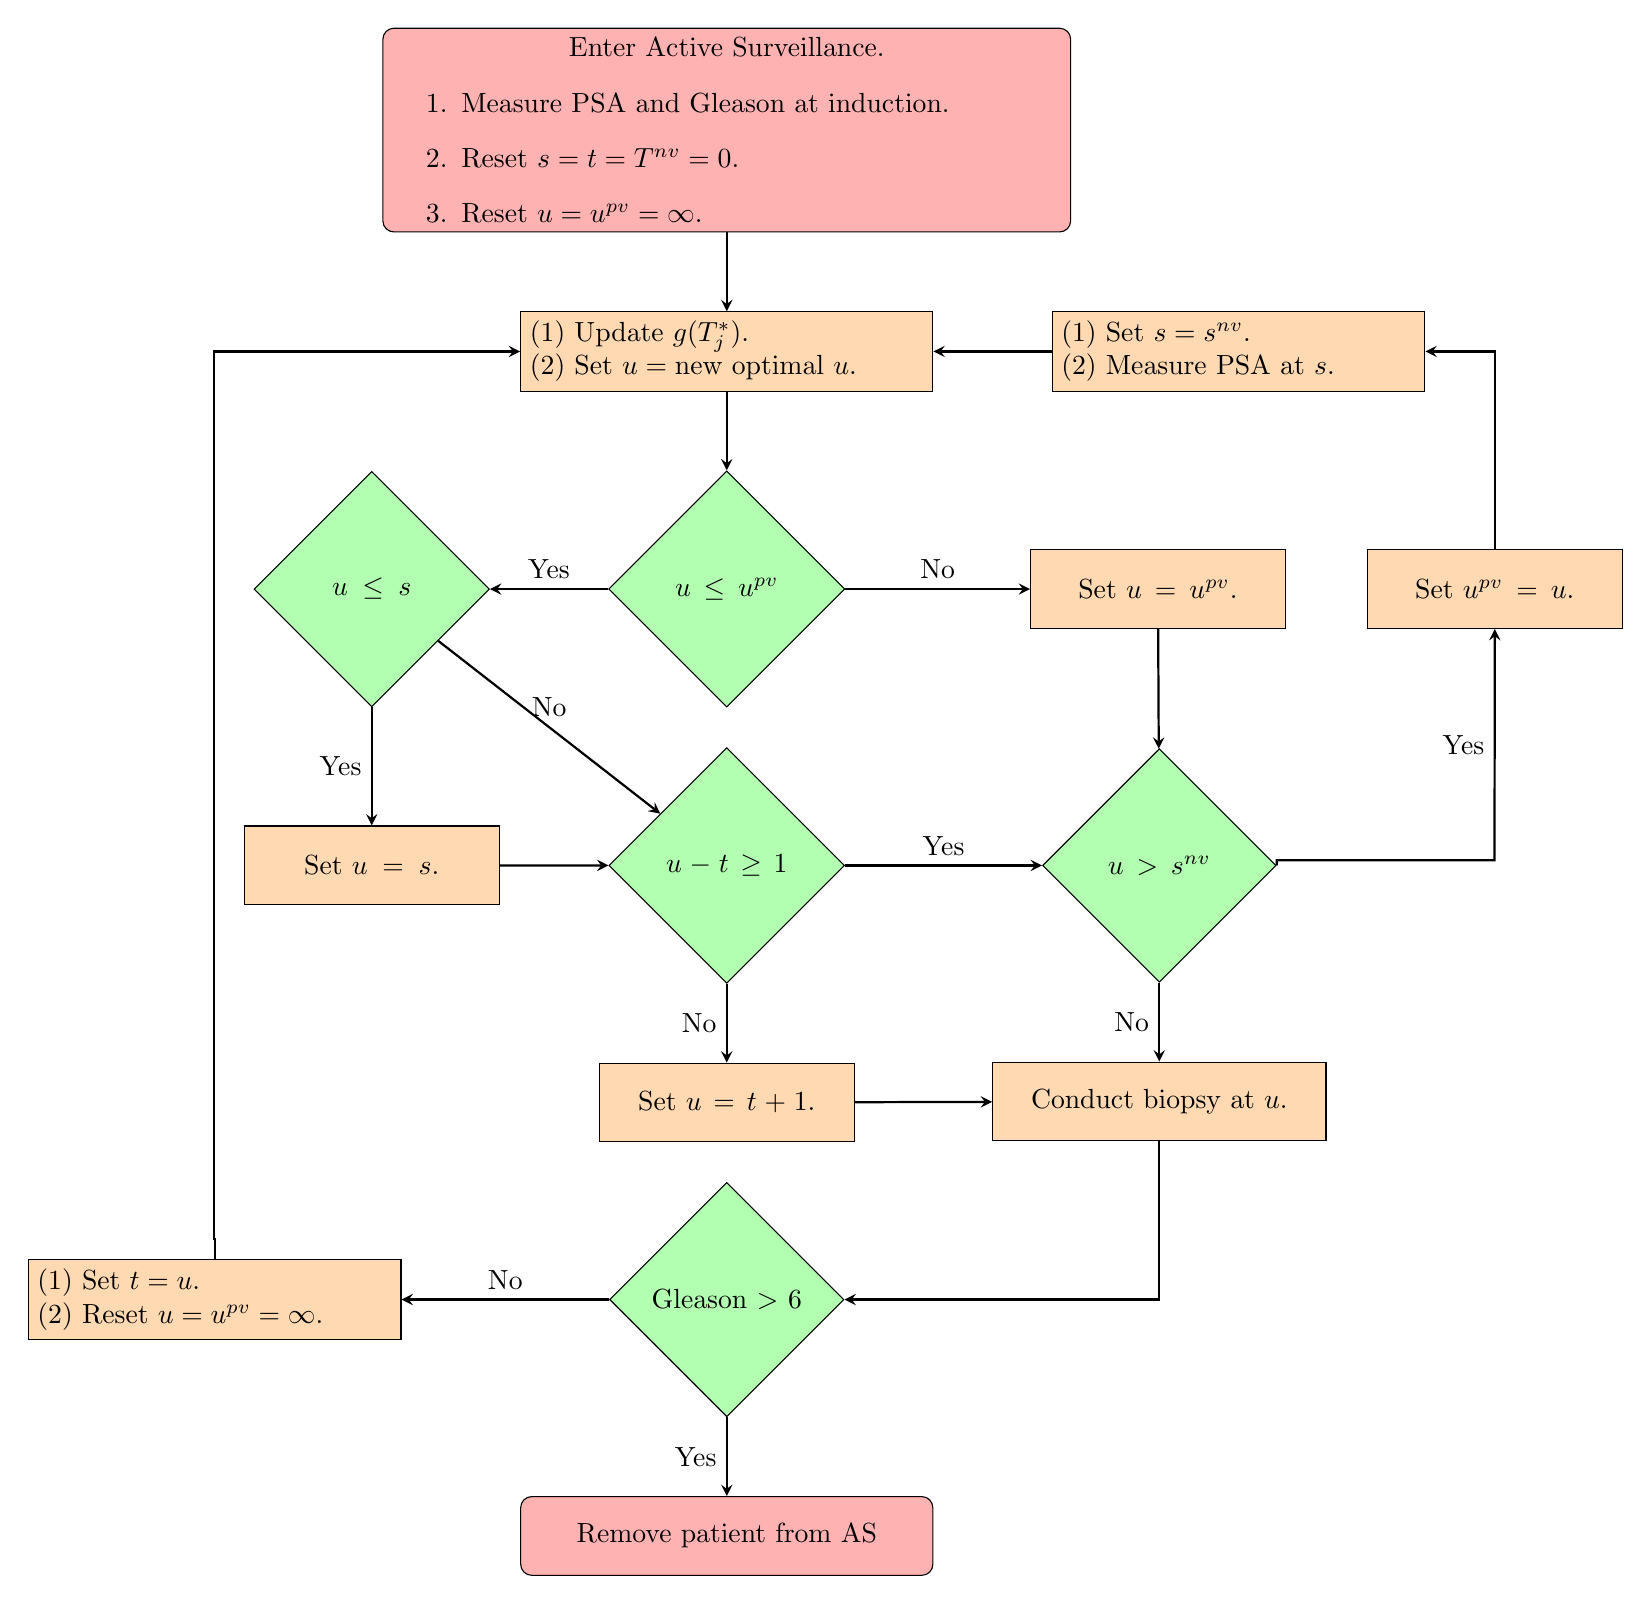
\begin{tikzpicture}
\node (start) [startstop_big] {
Enter Active Surveillance.
\begin{enumerate}
\item Measure PSA and Gleason at induction.
\item Reset $s=t=T^{nv}=0$. 
\item Reset $u = u^{pv} = \infty$.
\end{enumerate}
};

\node (propTime) [process_wide_5cm, below=1cm of start] {
(1) Update $g(T^*_j)$.\\
(2) Set $u = \mbox{new optimal } u$.
};

\node (decision1) [decision, below = 1.0cm of propTime] {$u \leq u^{pv}$};
\node (pro6) [process, right = 2.345cm of decision1] {Set $u = u^{pv}$.};

\node (takePSA) [process_wide_4pt5cm, right=1.5cm of propTime] {
(1) Set $s=s^{nv}$.\\
(2) Measure PSA at $s$. 
};


\node (decision5) [decision, left=1.5cm of decision1] {$u \leq s$};

\node (pro5) [process, below=1.5cm of decision5] {Set $u = s$.};

\node (decision2) [decision, below=0.5cm of decision1] {$u - t \geq 1$};

\node (decision4) [decision, right=2.5cm of decision2] {$u > s^{nv}$};

\node (pro8) [process, right=1.03cm of pro6] {Set $u^{pv}=u$.};

\node (pro3) [process, below=1.0cm of decision2] {Set $u = t + 1$.};

\node (pro4) [process_wide_4cm, below=1cm of decision4] {Conduct biopsy at $u$.};

\node (decision3) [decision, below=0.5cm of pro3] {$\mbox{Gleason} > 6$};
\node (pro7) [process_wide_4pt5cm, left=2.635cm of decision3] {
(1) Set $t = u$.\\
(2) Reset $u = u^{pv}=\infty$.
};

\node (stop) [startstop, below = 1cm of decision3] {Remove patient from AS};

\draw [arrow] (start) -- (propTime);
\draw [arrow] (takePSA) -- (propTime);
\draw [arrow] (propTime) -- (decision1);
\draw [arrow] (decision1) -- node[anchor=south] {Yes} (decision5);
\draw [arrow] (decision5) -- node[anchor=east] {Yes} (pro5);
\draw [arrow] (pro5) -- (decision2);
\draw [arrow] (decision1) -- node[anchor=south] {No} (pro6);
\draw [arrow] (decision5) -- node[anchor=south] {No} (decision2);
\draw [arrow] (pro6) -- (decision4);
\draw [arrow] (decision4.east) |- ([xshift=2.65cm, yshift=-3.95cm]pro6.north east) -- node[anchor=east] {Yes} (pro8);

\draw [arrow] (pro8) |- (takePSA);

\draw [arrow] (decision2) -- node[anchor=south] {Yes} (decision4);
\draw [arrow] (decision2) -- node[anchor=east] {No} (pro3);
\draw [arrow] (pro3) -- (pro4);
\draw [arrow] (pro4) |- (decision3);
\draw [arrow] (decision3) -- node[anchor=east] {Yes} (stop);
\draw [arrow] (decision4) -- node[anchor=east] {No} (pro4);
\draw [arrow] (decision3) -- node[anchor=south]{No} (pro7);
\draw [arrow] (pro7.north)|- ([xshift=-0.375cm, yshift=-5.25cm]pro5.north west) |- (propTime);
\end{tikzpicture}
}
}
%\caption{Algorithm for creating a personalized schedule for patient $j$. $t$ denotes the time of the latest biopsy. $s$ denotes the time of the latest available PSA measurement. $u$ denotes the proposed personalized time of biopsy.  $u^{pv}$ denotes the time at which a repeat biopsy was proposed on the last visit to the hospital. $T^{nv}$ denotes the time of the next visit for measurement of PSA.} 
%\label{fig : sched_algorithm}
%\end{figure*}
% !TEX root =  ../pers_schedules.tex

\section{Evaluation of Schedules}
\label{sec : choosing_schedule}
Given a particular schedule $S$ of biopsies, our next goal is to evaluate the schedule and to compare it with other schedules. To this end, we first present the methods to evaluate the biopsy schedules and then discuss the choice of a schedule.

We evaluate a schedule $S$ using two criteria, namely the number of biopsies $N^S_j \geq 1$ a schedule conducts for the $j$-th patient to detect GR, and the offset $O^S_j \geq 0$ by which it overshoots the true GR time $T^*_j$. The offset $O^S_j$ is defined as $O^S_j = T^S_{j{N^S_j}} - T^*_j$, where $T^S_{j{N^S_j}} \geq T^*_j$ is the time at which GR is detected. Our interest lies in the joint distribution $p(N^S_j, O^S_j)$ of the number of biopsies and the offset. Given the medical burden of biopsies, ideally only one biopsy with zero offset should be conducted. Hence, realistically we should select a schedule with a low mean number of biopsies $E(N^S_j)$ as well a low mean offset $E(O^S_j)$. It is also desired that a schedule has low variance of the number of biopsies $\mbox{var}(N^S_j)$, as well as low variance of the offset $\mbox{var}(O^S_j)$, so that the schedule works similarly for most patients. Quantiles of $p(N^S_j)$ may also be of interest. For example, it may be desired that a schedule detects GR with at most two biopsies in 95\% of the patients.

\subsection{Choosing a Schedule}
Given the multiple criteria for evaluation of a schedule, the next step is to use them to select a schedule. Using principles from compound optimal designs \citep{lauter1976optimal} we propose to choose a schedule $S$ which minimizes a loss function of the following form:
\begin{equation}
\label{eq : loss_func_sim_study_generic}
L(S) = \sum_{r=1}^R \eta_r \mathcal{R}_r(N^S_j).
\end{equation}
where $\mathcal{R}_r(\cdot)$ is an evaluation criteria based on either the number of biopsies or the offset (for brevity of notation, only $N^S_j$ is used in the equation above). Some examples of $\mathcal{R}_r(\cdot)$ are mean, median, variance and quantile function. Constants $\eta_1, \ldots, \eta_R$, where $0 \leq \eta_r \leq 1$ and $\sum_{r=1}^R \eta_r = 1$, are weights to differentially weigh-in the contribution of each of the $R$ criteria. An example loss function is:
\begin{equation}
\label{eq : loss_func_sim_study}
L(S) = \eta_1 E(N^S_j) + \eta_2 E(O^S_j). 
\end{equation}
The choice of $\eta_1$ and $\eta_2$ is not easy, because biopsies have associated medical risks and consequently the cost of an extra biopsy cannot be quantified or compared to a unit increase in offset easily. To obviate this problem we utilize the equivalence between compound and constrained optimal designs \citep{cook1994equivalence}. More specifically, it can be shown that for any $\eta_1$ and $\eta_2$ there exists a constant $C>0$ for which minimization of loss function in (\ref{eq : loss_func_sim_study}) is equivalent to minimization of the loss function subject to the constraint that $E(O^S_j) < C$. That is, a suitable schedule is the one which conducts the least number of biopsies to detect GR while simultaneously guaranteeing an offset less than $C$. The choice of $C$ now can be based on the protocol of AS program. In the more generic case in (\ref{eq : loss_func_sim_study_generic}), a schedule can be chosen by minimizing $\mathcal{R}_R(\cdot)$ under the constraint $\mathcal{R}_r(\cdot) < C_r; r=1, \ldots, R-1$.
% !TEX root =  ../pers_schedules.tex

\section{Demonstration of Personalized Schedules}
\label{sec : pers_schedule_PRIAS}
To demonstrate how the personalized schedules work, we apply them to the patients enrolled in PRIAS. To this end, we divide the PRIAS dataset into a training dataset with 5264 patients and a demonstration dataset with three patients who never experienced GR. We fit a joint model to the training dataset and then use it to create personalized schedules for patients in demonstration dataset. We fit the joint model using the R package \textbf{JMbayes} \citep{rizopoulosJMbayes}, which uses the Bayesian methodology to estimate the model parameters.

\subsection{Fitting the Joint Model to PRIAS Dataset}
\label{subsec : jm_fit_prias}
The training dataset contains age at the time of induction in PRIAS, PSA levels and the time interval in which GR is detected, for 5264 prostate cancer patients. PSA was measured at every three months for the first two years and every six months thereafter. To detect GR, biopsies were conducted as per the PRIAS schedule (Section \ref{sec : introduction}). For the longitudinal analysis of PSA we use $\log_2 \mbox{PSA}$ measurements instead of the raw data \citep{nieboer2015nonlinear}. The longitudinal sub-model of the joint model we fit is given by:
\begin{equation}
\label{eq : long_model_prias}
\begin{aligned}
\log_2 \mbox{PSA}(t) &= \beta_0 + \beta_1 (\mbox{Age}-70) + \beta_2 (\mbox{Age}-70)^2 + \sum_{k=1}^4 \beta_{k+2} B_k(t,\mathcal{K})\\ 
&+  b_{i0} + b_{i1} B_7(t, 0.1) + b_{i2} B_8(t, 0.1) +
\varepsilon_i(t).
\end{aligned}
\end{equation}
where $B_k(t, \mathcal{K})$ denotes the $k$-th basis function of a B-spline with three internal knots at $\mathcal{K} =\{0.1, 0.5, 4\}$ years, and boundary knots at zero and seven years. The spline for the random effects consists of one internal knot at 0.1 years and boundary knots at zero and seven years. The choice of knots was based on exploratory analysis as well as on model selection criteria AIC and BIC. Age of patients was median centered to avoid numerical instabilities during parameter estimation. For the relative risk sub-model the hazard function we fit is given by:
\begin{equation}
\label{eq : hazard_prias}
h_i(t) = h_0(t) \exp\big\{\gamma_1 (\mbox{Age}-70)  + \gamma_2 (\mbox{Age}-70)^2 + \alpha_1 m_i(t) + \alpha_2 m'_i(t)\big\}.
\end{equation}
where $\alpha_1$ and $\alpha_2$ are measures of strength of the association between hazard of GR and $\log_2 \mbox{PSA}$ value $m_i(t)$ and $\log_2 \mbox{PSA}$ velocity $m'_i(t)$, respectively. Since the PRIAS schedule depends only on the observed PSA values (via PSA-DT), the interval censoring observed in PRIAS is independent and non informative of the underlying health of the patient.

From the joint model fitted to the PRIAS dataset we found that only $\log_2 \mbox{PSA}$ velocity was strongly associated with hazard of GR. For any patient, a unit increase in $\log_2 \mbox{PSA}$ velocity led to an 11 fold increase in the hazard of GR. The parameter estimates for the fitted joint model are presented in detail in Web Appendix C of the supplementary material. 

\subsection{Personalized Schedules for the First Demonstration Patient}
\label{subsec : demo_prias_pers_schedule}
Using the demonstration dataset, we next present the functioning of personalized schedules based on expected time of GR and dynamic risk of GR. The evolution of PSA, time of last biopsy and proposed biopsy times for the first demonstration patient are shown in the top panel of Figure \ref{web_fig : prias_demo_pid_911}. We can see the combined effect of decreasing PSA levels and a negative repeat biopsy on personalized schedules, between year three and year 4.5 for this patient. In accordance with the two negative repeat biopsies and consistently decreasing PSA, the proposed time of biopsy based on dynamic risk of GR increases from 14 years to 15 years in this period. Whereas, the proposed time of biopsy based on expected time of GR increases from 16.6 years to 18.8 years. We can also see in the bottom panel of Figure \ref{web_fig : prias_demo_pid_911} that after each negative repeat biopsy, $\mbox{SD}[T^*_j] = \sqrt{\mbox{var}_g(T^*_j)}$ decreases sharply. Thus, if the expected time of GR based approach is used, then the offset $O^S_j$ will be smaller on average for biopsies scheduled after the second repeat biopsy than those scheduled after the first repeat biopsy.

\begin{figure}
\centerline{
\includegraphics[width=\columnwidth]{images/prias_demo/case_911.eps}
}
\caption{Top panel: Evolution of PSA, history of repeat biopsies and corresponding personalized schedules for the first demonstration patient. Bottom Panel: History of repeat biopsies and $\mbox{SD}_g(T^*_j) = \sqrt{\mbox{var}_g(T^*_j)}$ over time for the first demonstration patient.}
\label{web_fig : prias_demo_pid_911}
\end{figure}

The demonstration of personalized schedules for the two other patients from the demonstration data set is presented in Web Appendix D of the supplementary material.
% !TEX root =  ../pers_schedules.tex 
\section{Simulation Study}
\label{sec: simulation_study}
The application of personalized schedules for patients from PRIAS demonstrated that these schedules adapt according to the historical data of each patient. However we could not perform a full scale comparison between personalized and PRIAS schedule, because the true time of GR was not known for the PRIAS patients. To this end, we conducted a simulation study comparing personalized schedules with PRIAS and annual schedule, whose details are presented next.

\subsection{Simulation Setup}
\label{subsec : simulation_setup}
First we assume a population of patients enrolled in AS, with the same entrance criteria as that of PRIAS. The PSA and hazard of GR for patients from this population follow a joint model of the form postulated in Section \ref{subsec : jm_fit_prias}, with parameters equal to the posterior mean of parameters estimated from the joint model fitted to PRIAS dataset (Web Appendix C of the supplementary material). We further assume that there are three equal sized subgroups $G_1$, $G_2$ and $G_3$ of patients in the population, differing in the baseline hazard of GR. This was done because we wanted to test the performance of different schedules for a population with a mixture of patients, namely those with faster progressing PCa, as well as those with slowly progressing PCa. For the three subgroups we use a Weibull distributed baseline hazard with the following shape and scale parameters $(k, \lambda$): $(1.5, 4)$, $(3, 5)$ and $(4.5, 6)$ for $G_1, G_2$ and $G_3$, respectively. The effect of these parameters is that the mean GR time is lowest in $G_1$ (faster progressing PCa) and highest in $G_3$ (slowly progressing PCa).

From this population we have sampled 500 datasets with 1000 patients each. Patients are randomly assigned to a subgroup. Further, each dataset is split into a training (750 patients) and a test (250 patients) part. The $k$-th simulated training dataset $\mathcal{D}^k$ is given by $\mathcal{D}^k = \{l_{ki}, r_{ki}, \boldsymbol{y}_{ki}; i = 1, \ldots, 750\}$, where $\boldsymbol{y}_{ki}$ denote the PSA measurements for the $i$-th patient in $\mathcal{D}^k$. The frequency of PSA measurements is same as that in PRIAS. Other than simulating a true GR time $T^*_{ki}$, we also generate a random and non-informative censoring time $C_{ki}$. When $T^*_{ki} < C_{ki}$, then $l_{ki} = r_{ki} = T^*_{ki}$, otherwise $l_{ki} = C_{ki}$ and $r_{ki} = \infty$. For the test patients, censoring time is not generated.

We next fit a joint model of the specification given in (\ref{eq : long_model_prias}) and (\ref{eq : hazard_prias}) to each of the $\mathcal{D}^k, k=1, \ldots, 500$, and obtain a MCMC sample from the posterior distribution $p(\boldsymbol{\theta} \mid \mathcal{D}^k)$. We then obtain $g(T^*_{kl})$ for each of the $l$-th test patient of the $k$-th data set and conduct hypothetical biopsies for him. For every patient we conduct biopsies using the following six types of schedules (abbreviated names in parenthesis): personalized schedules based on expected time of GR (Exp. GR time) and median time of GR (Med. GR time), personalized schedules based on dynamic risk of GR (Dyn. risk GR), a hybrid approach between median time of GR and dynamic risk of GR (Hybrid), PRIAS schedule and annual schedule. The biopsies are conducted iteratively in accordance with the algorithm in Figure \ref{fig : sched_algorithm}. 

To compare the aforementioned schedules we require estimates of the various criteria based on offset and number of biopsies conducted to detect GR (Section \ref{sec : choosing_schedule}). To this end, we compute pooled estimates of each of the $E(N^S_j)$, $\mbox{var}(N^S_j)$, $E(O^S_j)$ and $\mbox{var}(O^S_j)$, as below:
\begin{align*}
\widehat{E(O^S_j)} &= \frac{\sum_{k=1}^{500} n_k \widehat{E(O^S_k)}}{\sum_{k=1}^{500} n_k}, \\
\widehat{\mbox{var}(O^S_j)} &= \frac{\sum_{k=1}^{500} (n_k - 1) \widehat{\mbox{var}(O^S_k)}}{\sum_{k=1}^{500} (n_k-1)}, 
\end{align*}
where $n_k$ denotes the number of test patients, $\widehat{E(O^S_k)} = {\sum_{l=1}^{n_k}O^S_{kl}}/{n_k}$ is the estimated mean and $\widehat{\mbox{var}(O^S_k)} = {\sum_{l=1}^{n_k}\big\{O^S_{kl} - \widehat{E(O^S_k)}\big\}^2}/(n_k-1)$ is the estimated variance of the offset for the $k$-th simulation. The estimates for number of biopsies are obtained similarly.

\subsection{Results}
The pooled estimates of the aforementioned criteria are summarized in Table \ref{table : sim_study_pooled_estimates}. In addition, mean offset is plotted against mean number of biopsies conducted to detect GR in Figure \ref{fig : meanNbVsOffset}. From the figure it is evident that across the schedules there is an inverse relationship between $E(N^S_j)$ and $E(O^S_j)$. For example, the annual schedule conducts on average 5.2 biopsies to detect GR, which is the highest among all schedules, however it has the least average offset of 6 months as well. On the other hand the schedule based on expected time of GR conducts only 1.9 biopsies on average to detect GR, the least among all schedules, but it also has the highest average offset of 15 months. The schedule based on median time of GR performs similar to that based on expected time of GR. Since the annual schedule attempts to contain the offset within an year it has the least $\mbox{SD}(O^S_j) = \sqrt{\mbox{var}(O^S_j)}$. However to achieve so, it conducts a wide range of number of biopsies from patient to patient, i.e., highest $\mbox{SD}(N^S_j) = \sqrt{\mbox{var}(N^S_j)}$. Schedules based on expected and median time of GR perform the opposite of annual schedule in terms of $\mbox{SD}(N^S_j)$ and $\mbox{SD}(O^S_j)$.

\begin{figure}
\centerline{\includegraphics[width=\columnwidth]{images/sim_study/meanNbVsOffset_all.eps}}
\caption{Estimated mean number of biopsies and mean offset (months) for the 6 schedules, using all simulated patients.}
\label{fig : meanNbVsOffset}
\end{figure}

%124781 = 41484 + 41423 + 41874
\begin{table}
\caption{Estimated mean and standard deviation of the number of biopsies and offset (months).}
\label{table : sim_study_pooled_estimates}
\begin{tabular}{lrrrr}
\Hline
\multicolumn{5}{c}{a) All subgroups}\\
\hline
Schedule          & $E(N^S_j)$ & $E(O^S_j)$ & ${\mbox{SD}(N^S_j)}$ & ${\mbox{SD}(O^S_j)}$ \\
\hline
Annual         & 5.24            & 6.01                & 2.53          & 3.46              \\
PRIAS          & 4.90            & 7.71                & 2.36          & 6.31\\
Dyn. risk GR       & 4.69            & 6.66                & 2.19           & 4.38              \\
Hybrid       & 3.75            & 9.70                & 1.71          & 7.25              \\
Med. GR time & 2.06            & 13.88               & 1.41          & 11.80              \\
Exp. GR time & 1.92            & 15.08               & 1.19          & 12.11             \\
\hline
\multicolumn{5}{c}{b) Subgroup $G_1$}\\
\hline
Schedule        & $E(N^S_j)$ & $E(O^S_j)$ & ${\mbox{SD}(N^S_j)}$ & ${\mbox{SD}(O^S_j)}$ \\
\hline
Annual         & 4.32            & 6.02                & 3.13          & 3.44              \\
PRIAS          & 4.07            & 7.44                & 2.88          & 6.11    \\
Dyn. risk GR       & 3.85            & 6.75                & 2.69          & 4.44              \\
Hybrid       & 3.25            & 10.25               & 2.16          & 8.07              \\
Med. GR time & 1.84            & 20.66               & 1.76          & 14.62             \\
Exp. GR time & 1.72            & 21.65               & 1.47          & 14.75             \\
\hline      
\multicolumn{5}{c}{c) Subgroup $G_2$}\\
\hline
Schedule        & $E(N^S_j)$ & $E(O^S_j)$ & ${\mbox{SD}(N^S_j)}$ & ${\mbox{SD}(O^S_j)}$ \\
\hline
Annual         & 5.18            & 5.98                & 2.13          & 3.47              \\
PRIAS          & 4.85            & 7.70                & 2.00          & 6.29        \\
Dyn. risk GR       & 4.63            & 6.66                & 1.82          & 4.37              \\
Hybrid       & 3.68            & 10.32                & 1.37          & 7.45              \\
Med. GR time & 1.89             & 12.33               & 1.16          & 9.44              \\
Exp. GR time & 1.77            & 13.54               & 0.98          & 9.83              \\
\hline      
\multicolumn{5}{c}{d) Subgroup $G_3$}\\
\hline
Schedule        & $E(N^S_j)$ & $E(O^S_j)$ & ${\mbox{SD}(N^S_j)}$ & ${\mbox{SD}(O^S_j)}$ \\
\hline
Annual         & 6.20             & 6.02                & 1.76          & 3.46              \\
PRIAS          & 5.76             & 7.98                & 1.71         & 6.51        \\
Dyn. risk GR       & 5.58            & 6.58                & 1.56          & 4.33              \\
Hybrid       & 4.32            & 8.55                & 1.26          & 5.91              \\
Med. GR time & 2.45            & 8.70                & 1.15          & 6.32              \\
Exp. GR time & 2.27            & 10.09               & 0.99          & 7.47              \\
\hline     
\end{tabular}
\end{table}

The PRIAS schedule conducts only 0.3 biopsies less than the annual schedule, but with a higher variance of offset, it does not guarantee early detection for everyone. If we compare the PRIAS schedule with dynamic risk of GR based schedule, we can see that the latter performs slightly better than PRIAS schedule in all four criteria. The hybrid approach combines the benefits of methods with low $E(N^S_j)$ and $\mbox{SD}(N^S_j)$, and methods with low $E(O^S_j)$ and $\mbox{SD}(O^S_j)$. It conducts 1.5 biopsies less than the annual schedule on average and with a $E(O^S_j)$ of 9.7 months it detects GR within an year since its occurrence. Moreover, it has both $\mbox{SD}(N^S_j)$ and $\mbox{SD}(O^S_j)$ comparable to PRIAS.

The performance of each schedule differs for the three subgroups $G_1, G_2$ and $G_3$. The annual schedule remains the most consistent across subgroups in terms of the offset, but it conducts 2 extra biopsies for subgroup $G_3$ (slowly progressing PCa) than $G_1$ (faster progressing PCa). The performance of schedule based on expected time of GR is the most consistent in terms of number of biopsies but it detects GR an year later on average in subgroup $G_1$ than $G_3$. For the dynamic risk of GR based schedule and the hybrid schedule the dynamics are similar to that of the annual schedule. Unlike the latter two schedules, the PRIAS schedule not only conducts more biopsies in $G_3$ than $G_1$ but also detects GR later in $G_3$ than $G_1$.

\begin{figure}[!htb]
\centerline{\includegraphics[width=\columnwidth]{images/sim_study/nbBoxPlot_all.eps}}
\caption{Boxplot showing variation in number of biopsies conducted by different methods, using all simulated patients.}
\label{fig : nbBoxPlot_all}
\end{figure}

\begin{figure}[!htb]
\centerline{\includegraphics[width=\columnwidth]{images/sim_study/offsetBoxPlot_all.eps}}
\caption{Boxplot showing variation in biopsy offset (months) for different methods, using all simulated patients.}
\label{fig : offsetBoxPlot_all}
\end{figure}

The choice of a suitable schedule using (\ref{eq : loss_func_sim_study_generic}) depends on the chosen criteria for evaluation of schedules. For example, the schedule based on dynamic risk of GR is suitable if on average the least number of biopsies are to be conducted to detect GR, while simultaneously making sure that at least 90\% of the patients have an average offset less than one year (Figure \ref{fig : nbBoxPlot_all} and \ref{fig : offsetBoxPlot_all}). The schedule based on expected time of GR is suitable if on average the least number of biopsies are to be conducted to detect GR, while simultaneously making sure that at least 90\% of the patients have an average offset less than three years. If a stricter cutoff is required on offset the hybrid approach may be suitable, since it conducts only 3.8 biopsies on average while guaranteeing an offset of two years for 95\% of the patients and three years for 99.9\% of the patients. Besides if further cutoffs are required on variance of number of biopsies or offset they are not too high either for the hybrid approach.
\mySection{Related Works and Discussion}{}
\label{chap3:sec:discussion}

In this section we briefly discuss the similarities and differences of the model presented in this chapter, comparing it with some related work presented earlier (Chapter \ref{chap1:artifact-centric-bpm}). We will mention a few related studies and discuss directly; a more formal comparative study using qualitative and quantitative metrics should be the subject of future work.

Hull et al. \citeyearpar{hull2009facilitating} provide an interoperation framework in which, data are hosted on central infrastructures named \textit{artifact-centric hubs}. As in the work presented in this chapter, they propose mechanisms (including user views) for controlling access to these data. Compared to choreography-like approach as the one presented in this chapter, their settings has the advantage of providing a conceptual rendezvous point to exchange status information. The same purpose can be replicated in this chapter's approach by introducing a new type of agent called "\textit{monitor}", which will serve as a rendezvous point; the behaviour of the agents will therefore have to be slightly adapted to take into account the monitor and to preserve as much as possible the autonomy of agents.

Lohmann and Wolf \citeyearpar{lohmann2010artifact} abandon the concept of having a single artifact hub \cite{hull2009facilitating} and they introduce the idea of having several agents which operate on artifacts. Some of those artifacts are mobile; thus, the authors provide a systematic approach for modelling artifact location and its impact on the accessibility of actions using a Petri net. Even though we also manipulate mobile artifacts, we do not model artifact location; rather, our agents are equipped with capabilities that allow them to manipulate the artifacts appropriately (taking into account their location). Moreover, our approach considers that artifacts can not be remotely accessed, this increases the autonomy of agents.

The process design approach presented in this chapter, has some conceptual similarities with the concept of \textit{proclets} proposed by Wil M. P. van der Aalst et al. \citeyearpar{van2001proclets, van2009workflow}: they both split the process when designing it. In the model presented in this chapter, the process is split into execution scenarios and its specification consists in the diagramming of each of them. Proclets \cite{van2001proclets, van2009workflow} uses the concept of \textit{proclet-class} to model different levels of granularity and cardinality of processes. Additionally, proclets act like agents and are autonomous enough to decide how to interact with each other.

The model presented in this chapter uses an attributed grammar as its mathematical foundation. This is also the case of the AWGAG model by Badouel et al. \citeyearpar{badouel14, badouel2015active}. However, their model puts stress on modelling process data and users as first class citizens and it is designed for Adaptive Case Management.

To summarise, the proposed approach in this chapter allows the modelling and decentralized execution of administrative processes using autonomous agents. In it, process management is very simply done in two steps. The designer only needs to focus on modelling the artifacts in the form of task trees and the rest is easily deduced. Moreover, we propose a simple but powerful mechanism for securing data based on the notion of accreditation; this mechanism is perfectly composed with that of artifacts. The main strengths of our model are therefore : 
\begin{itemize}
	\item The simplicity of its syntax (process specification language), which moreover (well helped by the accreditation model), is suitable for administrative processes;
	\item The simplicity of its execution model; the latter is very close to the blockchain's execution model \cite{hull2017blockchain, mendling2018blockchains}. On condition of a formal study, the latter could possess the same qualities (fault tolerance, distributivity, security, peer autonomy, etc.) that emanate from the blockchain;
	\item Its formal character, which makes it verifiable using appropriate mathematical tools;
	\item The conformity of its execution model with the agent paradigm and service technology.
\end{itemize}
In view of all these benefits, we can say that the objectives set for this thesis have indeed been achieved. However, the proposed model is perfectible. For example, it can be modified to permit agents to respond incrementally to incoming requests as soon as any prefix of the extension of a bud is produced. This makes it possible to avoid the situation observed on figure \ref{chap3:fig:execution-figure-4} where the associated editor is informed of the evolution of the subtree resulting from $C$ only when this one is closed. All the criticisms we can make of the proposed model in particular, and of this thesis in general, have been introduced in the general conclusion (page \pageref{chap5:general-conclusion}) of this manuscript.




\section{Acknowledgement}
\label{sec:conclusion}
This work is supported by National Natural Science Foundation of China (62076144), Shenzhen Key Laboratory of next generation interactive media innovative technology (ZDSYS20210623092001004),\\ Shenzhen Science and Technology Program (WDZC2022081614051\\5001) and Tencent AI Lab Rhino-Bird Focused Research Program (RBFR2022005).

\section*{Supplementary Materials}

Web Appendix A, C, D and E referenced in Section~\ref{sec : jm_framework},  Section~\ref{sec : pers_schedule_PRIAS},  and  Section~\ref{sec: discussion}, respectively, and the derivation of Equation (\ref{eq : expected_time_survprob}) and (\ref{eq : var_time_survprob}) in Web Appendix B, are available in a supplementary document uploaded at \url{https://goo.gl/jpPtL8}.\vspace*{-8pt}

\textbf{}

\clearpage
\printbibliography

\appendix

\end{document}